\scanpage{3}
\mspage{1}
\uline{On certain graded rings}

\inserted{Let $k$ be a fixed (\unsure{commutative|commutative}) ring.}

1. \unsure{Let|Let} \deleted{$k$ be a ring,} $M^*$ be a graded $k$-module\inserted{\figure{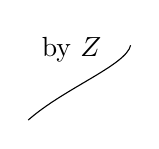
\begin{tikzpicture}[x=1cm,y=1cm]\node at (0,.35) {by $\mathbb Z$};\draw (-.55,-.55) .. controls (-.1,-.15) and (.7,.15) .. (.75,.4);\end{tikzpicture}}}, \inserted{\figure{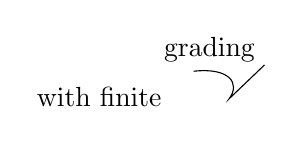
\begin{tikzpicture}[x=1cm,y=1cm]\node at (0,.05) {with finite};\node at (1.4,.65) {grading};\draw (1.2,.37) .. controls (1.65,.42) and (1.8,.22) .. (1.65,.02)--(2.1,.45);\end{tikzpicture}}}, $\mathcal E^*$ a \deleted{graded algebra}\inserted{\figure{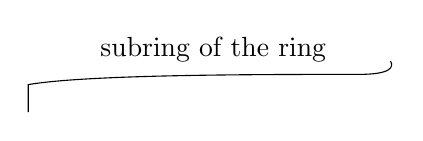
\begin{tikzpicture}[x=1cm,y=1cm]\node at (0,.35) {subring of the ring};\draw (-2.35,-.45)--(-2.35,-.1) .. controls (-1.6,.03) and (.6,.03) .. (1.85,.03) .. controls (2.25,.03) and (2.3,.12) .. (2.25,.2);\end{tikzpicture}}} of endomorphisms \inserted{\figure{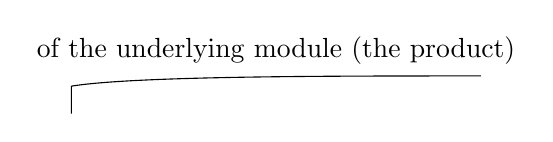
\begin{tikzpicture}[x=1cm,y=1cm]\node at (0,.35) {of the underlying module (the product)};\draw (-2.6,-.45)--(-2.6,-.1) .. controls (-1.8,.03) and (.7,.03) .. (2.6,.03);\end{tikzpicture}}} of $M^*$. We denote by $\pi_i$ the canonical projection of $M^*$ onto $M^i$. \deleted{and} We assume that we have:
\[
\pi_i\in\mathcal E^*\quad\text{for every }i
\tag{1.2}
\]
This implies that $\mathcal E^*$ is a graded \uline{sub-}\deleted{\uline{algebra}}\inserted{ring} of the graded algebra \deleted{of the} $\operatorname{End}(M^*)$ [whose grading is defined, if $\nu\in\mathbb Z$, by
\[
\operatorname{End}^{(\nu)}(M)=\sum\operatorname{Hom}(M^i,M^{i+\nu})
\]
or equivalently
\[
\operatorname{End}^{(\nu)}(M)=\sum_i\pi_{i+\nu}\operatorname{End}(M^*)\pi_i,
\]
the homogeneous component of degree $\nu$ of an endomorphism $u$ of $M^*$ being
\[
\deleted{\mathrm{gr}}\quad\operatorname{pr}_{\nu}(u)=\sum_i\pi_{i+\nu}u\pi_i.
\]
The grading of $\mathcal E^*$ is defined \inserted{\figure{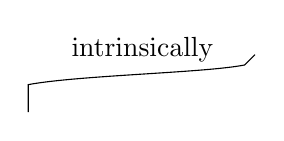
\begin{tikzpicture}[x=1cm,y=1cm]\node at (0,.35) {intrinsically};\draw (-1.45,-.45)--(-1.45,-.1) .. controls (-.8,.02) and (.8,.05) .. (1.3,.15)--(1.43,.28);\end{tikzpicture}}}, in terms of the \deleted{by} datum of the $\pi_i$, by
\[
\left\{\begin{aligned}
\text{\textcircled{a}}\quad&\boxed{\mathcal E^{(\nu)}=\sum_i\pi_{i+\nu}\mathcal E^*\pi_i}\,,\\
\text{\textcircled{b}}\quad&\operatorname{pr}_{\nu}^{\mathcal E}u=\sum_i\pi_{i+\nu}u\pi_i
\end{aligned}\right.
\tag{1.3}
\]
\margin{and $(1.4.)\quad u\in\mathcal E^{(\nu)}\Longleftrightarrow u\pi_i=\pi_{i+\nu}u$ for every $i$\par
$\deleted{\unsure{\Longleftrightarrow u=\pi_{i+\nu}u\pi_i}}$}
\margin{\figure{\begin{tikzpicture}[x=1cm,y=1cm]
\node[anchor=west] at (9.8,1.7) {Note the relations};
\node[anchor=west] at (.2,.8) {$(1.1)$};
\node[anchor=west] at (.2,.25) {\deleted{Let us note}};
\node[anchor=west] at (2.1,.55) {$\left\{\begin{aligned}\pi_i^2&=\pi_i\\\pi_i\pi_j&=0\quad\text{if }i\neq j\\\sum\pi_i&=1\end{aligned}\right.$};
\draw[draw=brown!60!black] (.25,1.35) .. controls (-.1,1.15) and (-.35,.25) .. (.05,.05) .. controls (2,-.4) and (8,-.2) .. (11.5,.1) .. controls (13.8,.2) and (14.2,1.7) .. (13.2,2.0) .. controls (11.5,2.15) and (6.8,1.2) .. (.65,1.32);
\draw[draw=brown!60!black] (.3,1.15)--(.1,.65);
\draw[draw=brown!60!black] (.1,.6) circle (.055);
\end{tikzpicture}}}

2. Let $\mathcal E^*$ be a graded \deleted{$k$-algebra}\inserted{ring}, and let $\pi_i$ ($i\in\mathbb Z$) be elements of $\mathcal E$, \inserted{\figure{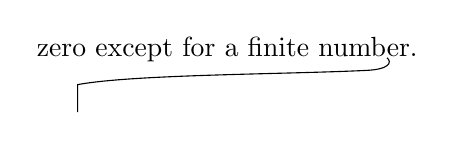
\begin{tikzpicture}[x=1cm,y=1cm]\node at (0,.35) {zero except for a finite number.};\draw (-1.9,-.45)--(-1.9,-.1) .. controls (-1.2,.03) and (.7,.03) .. (1.75,.08) .. controls (2.05,.09) and (2.1,.18) .. (2.03,.24);\end{tikzpicture}}} Under what conditions do the formulas $(1.3)$ define
\mspage{2}
